% Initial version by Darian Muresan, Ph.D.
% dmuresan@stevens.edu
% Edit and adjust as needed.
\documentclass[12pt]{cornell}
\usepackage[dvipsnames,table]{xcolor}


% add index support
%\usepackage{imakeidx}
\usepackage{makeidx}
%\makeindex

%--- ADDED BY CARSON ---
% \usepackage{appendix}
\usepackage{hhline}
%\usepackage{multirow}
%-----------------------

% graphing programs
\usepackage[dvipsnames]{color}
\usepackage{psfrag}
\usepackage{verbatim}
\usepackage{fancyhdr}
%\usepackage{titlesec}
\usepackage{fancyvrb} 
% hyperlink programs
%\usepackage{url}

% Does not work with LaTeX=>PDF
\usepackage[pdfmark, 
breaklinks=true, 
colorlinks=true,
citecolor=blue,
linkcolor=blue,
menucolor=black,
pagecolor=black,
urlcolor=blue
]{hyperref} % links in pdf

%\usepackage[colorlinks]{hyperref} % links in dvi
\usepackage{listings}
\usepackage{amsfonts} 
\usepackage{amssymb} 
%\usepackage{tabto}

\usepackage{tabularx,colortbl}
\usepackage[chapter]{algorithm} 
\usepackage{algorithmic} 
\usepackage{blindtext}

\definecolor{DarkGreen}{rgb}{0,0.6,0}
\definecolor{mygreen}{rgb}{0,0.6,0}
\definecolor{mygray}{rgb}{0.5,0.5,0.5}
\definecolor{mymauve}{rgb}{0.58,0,0.82}

\usepackage{tocloft}
\usepackage{amsmath}
\usepackage{tcolorbox}
\usepackage{enumitem}
\usepackage{longtable}
%\usepackage{textcomp}
\usepackage{txfonts}

%part for \part titles
%chap for \chapter titles
%sec for \section titles
%subsec for \subsection titles
%subsubsec for \subsubsection titles
%para for \paragraph titles
%subpara for \subparagraph titles
%fig for figure \caption titles
%subfig for subfigure \caption titles
%tab for table \caption titles
%subtab for subtable \caption titles


% update chapter number spacing
\setlength{\cftchapnumwidth}{2em}
\setlength{\cftsecnumwidth}{2.5em}
\setlength{\cftsubsecnumwidth}{3.5em}
\setlength{\cftsubsubsecnumwidth}{4.5em}

\addtolength{\cftsecindent}{0.5em}
\addtolength{\cftsubsecindent}{0.5em}
\addtolength{\cftsubsubsecindent}{0.5em}

%\titlespacing*{\chapter}{0pt}{-50pt}{20pt}
%\titleformat{\chapter}[display]{\normalfont\huge\bfseries}{\chaptertitlename\ 
%\thechapter}{20pt}{\Huge}
%\pagestyle{fancy}
%\pagestyle{cornell}
%
%\rhead{F054-021-0172}
%\chead{Nonlinear Enhancement of Visual Target Detection (AF05-T021)}
%\lhead{GSTI}
%\lfoot{\scriptsize Use or disclosure of data on this page is subject
%to the restriction on the title page of this proposal.}
%\cfoot{}
%\rfoot{\thepage}

\newfont{\Bp}{msbm10}
\newfont{\BpBig}{msbm10 scaled\magstep2}
\newfont{\Sc}{eusm10}
\newfont{\ScBig}{eusm10 scaled\magstep3}
\newfont{\Fr}{eufm10}
\newfont{\FrBig}{eufm10 scaled\magstep1}

% some commands:
\newcommand{\dxi}{{\tt m\_xDeltaInput}}
\newcommand{\dyi}{{\tt m\_yDeltaInput}}
\newcommand{\dci}{{\tt m\_cDeltaInput}}
\newcommand{\dxo}{{\tt m\_xDeltaOutput}}
\newcommand{\dyo}{{\tt m\_yDeltaOutput}}
\newcommand{\dco}{{\tt m\_cDeltaOutput}}
\newcommand{\ttf}[1]{{\tt #1}}
\newcommand{\tbl}[2]{{\begin{tabular}{c} #1 \\ #2 \end{tabular}}}

\newcommand{\urltwo}[2]{\mbox{\href{#1}{\tt #2}}}
\newcommand{\qnorm}[1]{\|#1\|_{\bQ}}
\newcommand{\qdot}[2]{\lrb #1, #2 \rrb_{\bQ}}
\newcommand{\kdot}[2]{\lrb #1, #2 \rrb_{\bf k}}
\newcommand{\tdot}[2]{\lrb #1, #2 \rrb}
\newcommand{\mydiff}[2]{\lrb #1 - #2 \rrb}
\newcommand{\lena}{\textit{lena}}
\newcommand{\barb}{\textit{barbara}}
\newcommand{\boat}{\textit{boat}}
\newcommand{\leaves}{\textit{leaves}}
\newcommand{\rings}{\textit{rings}}
\newcommand{\treg}{\textit{train region}}
\newcommand{\dreg}{\textit{denoise region}}
\newcommand{\oreg}{\textit{overlap region}}
\newcommand{\sil}{\sigma_l^2}
\newcommand{\sn}{\sigma^2}
\newcommand{\bn}{{\mbox{\bf \FrBig N}}}
\newcommand{\n}{\mbox{\Fr N}}
%\newcommand{\bn}{\bf N}
%\newcommand{\n}{N}
\newcommand{\bY}{\textbf{Y}}
\newcommand{\bX}{\textbf{X}}
\newcommand{\bb}{\textbf{b}}
\newcommand{\bu}{\textbf{u}}
\newcommand{\bv}{\textbf{v}}
\newcommand{\by}{\textbf{y}}
\newcommand{\bx}{\textbf{x}}
\newcommand{\be}{\textbf{e}}
\newcommand{\bz}{\textbf{z}}
\newcommand{\bs}{\textbf{s}}
\newcommand{\bw}{\textbf{w}}
\newcommand{\bQ}{\textbf{Q}}
\newcommand{\bphi}{\textbf{$\phi$}}
\newcommand{\lsb}{\left[}
\newcommand{\rsb}{\right]}
\newcommand{\lrb}{\left(}
\newcommand{\rrb}{\right)}
\newcommand{\lcb}{\left\{}
\newcommand{\rcb}{\right\}}
\newcommand{\R}{\mbox{\BpBig R}}
\newcommand{\F}{{\cal F}}
\newcommand{\Fk}{\mbox{\Sc F}}
\newcommand{\bQF}{\textbf{Q}_{\mbox{\Sc F}}}
\newcommand{\N}{{\cal N}}
\newcommand{\xlz}{X_l(z)}
\newcommand{\xhz}{X_h(z)}
\newcommand{\xz}{X(z)}
\newcommand{\pr}{ perfect reconstruction }
\newcommand{\smb}{Smith-Barnwell }
\newcommand{\xw}{X(e^{j\omega})}
\newcommand{\xmw}{X(-e^{j\omega})}
\newcommand{\dw}{D(e^{j\omega})}
\newcommand{\dmw}{D(-e^{j\omega})}
\newcommand{\ew}{E(e^{j\omega})}
\newcommand{\emw}{E(-e^{j\omega})}
\newcommand{\fw}{F_0(e^{j\omega})}
\newcommand{\fmw}{F_0(-e^{j\omega})}
\newcommand{\hoz}{H_1(z)}
\newcommand{\hzz}{H_0(z)}
\newcommand{\goz}{G_1(z)}
\newcommand{\gzz}{G_0(z)}
\newcommand{\hzw}{H_{0}(e^{j\omega})}
\newcommand{\hzmw}{H_{0}(-e^{j\omega})}
\newcommand{\hzcw}{H_{0}(e^{-j\omega})}
\newcommand{\how}{H_1(e^{j\omega})}
\newcommand{\homw}{H_1(-e^{j\omega})}
\newcommand{\gzw}{G_0(e^{j\omega})}
\newcommand{\gzmw}{G_0(-e^{j\omega})}
\newcommand{\gow}{G_1(e^{j\omega})}
\newcommand{\gomw}{G_1(-e^{j\omega})}
\newcommand{\wl}{e^{-jwL}}
\newcommand{\aqua}{\textit{AQua with OR }}
\newtheorem{theorem}{Theorem}
\newtheorem{lemma}{Lemma}
\newtheorem{corollary}{Corollary}
\newtheorem{claim}{Claim}
\newtheorem{definition}{Definition}
\newenvironment{proof}{\noindent{\em Proof.}}{\ \hfill Q.E.D.}
%\newtheorem{moduleCount}{L}
\newcommand*{\labelfile}[1]{%
  \label{file:#1}%
}

% Use this to label requirements, use cases, user stories, etc.
% This is where we can add different spellings for different types of 
% requirements, use cases, user stories, etc.
% \newtheorem{requirementKind}{Requirement Spelling}
\newtheorem{reqkFunctional}{Functional Requirement}
\newtheorem{reqkQuality}{Quality Requirement}
\newtheorem{reqkUser}{User Requirement}
\newtheorem{reqkUserConstraint}{User Constraint}
\newtheorem{reqkConstraint}{Constraint Requirement}
\newtheorem{reqkInterface}{Interface Requirement}
\newtheorem{reqkBusiness}{Business Requirement}
% Use cases
\newtheorem{useCase}{Use Case}
% User story
\newtheorem{userStory}{User Story}

% command for adding a version to the document
\newcommand{\VERSION}{Version 1.0.0}

% Family -- enter the name of the family that it belongs to: Chapter, Figure, Table, etc.
% Name -- name of the family member: file name, table name, etc.
\newcommand{\FamilyName}[2]{\hyperref[#1::#2]{#2}\index{#2}\xspace}
% Family -- same as above
% Name -- same as above
% Reference -- shorthand for the 'Name'.  It will show as Reference_NameID
% Kind -- underscore(_), space, or dash (-)
\newcommand{\FamilyNameReferenceKind}[4]{\hyperref[#1::#2]{$#3#4{\ref*{#1::#2}}$}}
% newcommand{Family,Label}
\newcommand{\FamilyLabel}[2]{\label{#1::#2}}


% for use cases
\newcommand{\UseCaseLabel}[1]{\FamilyLabel{UseCase}{#1}}
\newcommand{\UseCaseName}[1]{\FamilyName{UseCase}{#1}}
\newcommand{\UseCaseReference}[1]{\FamilyNameReferenceKind{UseCase}{#1}{UC}{_}}
% UseCase name with stacked reference
\newcommand{\UseCaseNameWSReference}[1]{\begin{tabular}{c}\UseCaseName{#1} \\ (\UseCaseReference{#1}) \end{tabular}}
% UseCase name with inline reference
\newcommand{\UseCaseNameWIReference}[1]{\UseCaseName{#1} (\UseCaseReference{#1})}

% for chapters
\newcommand{\ChapterName}[1]{\FamilyName{Chapter}{#1}}
\newcommand{\ChapterLabel}[1]{\FamilyLabel{Chapter}{#1}}
\newcommand{\ChapterReference}[1]{\FamilyNameReferenceKind{Chapter}{#1}{Chapter}{\mbox{ }}}
% Chapter name with inline (WI) reference 
\newcommand{\ChapterNameWIReference}[1]{\ChapterName{#1} (\ChapterReference{#1})}

% for figures
\newcommand{\FigureName}[1]{\FamilyName{Figure}{#1}}
\newcommand{\FigureLabel}[1]{\FamilyLabel{Figure}{#1}}
\newcommand{\FigureReference}[1]{\FamilyNameReferenceKind{Figure}{#1}{Figure}{\mbox{ }}}
% Figure name with stacked (WS) reference
\newcommand{\FigureNameWSReference}[1]{\begin{tabular}{c}\FigureName{#1} \\ (\FigureReference{#1}) \end{tabular}}
% Figure name with inline (WI) reference 
\newcommand{\FigureNameWIReference}[1]{\FigureName{#1} (\FigureReference{#1})}

% for tables
\newcommand{\TableName}[1]{\FamilyName{Table}{#1}}
\newcommand{\TableLabel}[1]{\FamilyLabel{Table}{#1}}
\newcommand{\TableReference}[1]{\FamilyNameReferenceKind{Table}{#1}{Table}{\mbox{ }}}

% for requirements
% RequirementLabel[Kind][Label]
\newcommand{\RequirementLabel}[2]{\FamilyLabel{#1}{#2}}
\newcommand{\RequirementName}[2]{\FamilyName{#1}{#2}}
\newcommand{\RequirementReference}[2]{\FamilyNameReferenceKind{#1}{#2}{#1}{_}}
% Requirements name with stacked (WS) reference
\newcommand{\RequirementNameWSReference}[2]{\begin{tabular}{c}\RequirementName{#1}{#2} \\ (\RequirementReference{#1}{#2}) \end{tabular}}
% Requirements name with inline (WI) reference 
\newcommand{\RequirementNameWIReference}[2]{\RequirementName{#1}{#1} (\RequirementReference{#1}{#2})}

% for requirements
% RequirementLabel[Kind][Label]
\newcommand{\UserStoryLabel}[2]{\FamilyLabel{#1}{#2}}
\newcommand{\UserStoryName}[2]{\FamilyName{#1}{#2}}
\newcommand{\UserStoryReference}[2]{\FamilyNameReferenceKind{#1}{#2}{R}{_}}
% Requirements name with stacked (WS) reference
\newcommand{\UserStoryNameWSReference}[2]{\begin{tabular}{c}\RequirementName{#1}{#2} \\ (\RequirementReference{#1}{#2}) \end{tabular}}
% Requirements name with inline (WI) reference 
\newcommand{\UserStoryNameWIReference}[2]{\RequirementName{#1}{#1} (\RequirementReference{#1}{#2})}


\definecolor{mygray}{gray}{0.9}
\lstset{ %
  backgroundcolor=\color{mygray},   % choose the background color; you must add \usepackage{color} or \usepackage{xcolor}
  basicstyle=\fontfamily{cmss}\footnotesize,        % the size of the fonts that are used for the code
  breakatwhitespace=false,         % sets if automatic breaks should only happen at whitespace
  breaklines=true,                 % sets automatic line breaking
  captionpos=b,                    % sets the caption-position to bottom
  commentstyle=\color{DarkGreen},    % comment style
  deletekeywords={...},            % if you want to delete keywords from the given language
  escapeinside={\%*}{*)},          % if you want to add LaTeX within your code
  extendedchars=true,              % lets you use non-ASCII characters; for 8-bits encodings only, does not work with UTF-8
  frame=L,                   % adds a frame around the code
  keepspaces=true,                 % keeps spaces in text, useful for keeping indentation of code (possibly needs columns=flexible)
  keywordstyle=\color{blue},       % keyword style
  language=Python,                    % the language of the code
  morekeywords={*,...},            % if you want to add more keywords to the set
  numbers=left,                    % where to put the line-numbers; possible values are (none, left, right)
  numbersep=10pt,                   % how far the line-numbers are from the code
  numberstyle=\tiny\color{gray}, % the style that is used for the line-numbers
  rulecolor=\color{black},         % if not set, the frame-color may be changed on line-breaks within not-black text (e.g. comments (green here))
  showspaces=false,                % show spaces everywhere adding particular underscores; it overrides 'showstringspaces'
  showstringspaces=false,          % underline spaces within strings only
  showtabs=false,                  % show tabs within strings adding particular underscores
  stepnumber=1,                    % the step between two line-numbers. If it's 1, each line will be numbered
  stringstyle=\color{mymauve},     % string literal style
  %tabsize=2,                      % sets default tabsize to 2 spaces
  %caption=\lstname                % show the filename of files included with \lstinputlisting; also try caption instead of title
  xleftmargin=\parindent
}


% Uncomment draftcopy to get the word DRAFT boldly across the first page
%   By the way, xdvi won't show it but it will come out when you print
%\usepackage[light,all]{draftcopy}		% DRAFT on first page
%\draftcopySetGrey{.97}
%\draftcopyName{Confidential}{150}
%\draftcopFirstPage{1}

% Uncomment drafthead to get the date and DRAFT in the header of pages
% that are normallly numbered on the top, pages 2-n of each chapter for example
% This doesn't work with centered page numbers: \pagestyle{cornellc}
%\usepackage{drafthead}

% glossaries to organize the document glossary
\usepackage{glossaries}

% glossary creation
\label{Chapter::Glossary}
\newglossaryentry{must}
{	name={MustHave},
	description={This defines the first highest priority requirement.
	All of the tasks, requirements, or anything that is marked this way are
	build in the current version}
}

\newglossaryentry{should}
{	name={ShouldHave},
	description={This defines the second highest priority requirement. The system should implement 
	all of the tasks, requirements, or anything that is marked this way, but if 
	resources are limited, it can be left out of the current version.
	Build in next version}
}

\newglossaryentry{could}
{	name={CouldHave},
	description={This defines the third highest priority requirement.The system could implement 
	all of the tasks, requirements, or anything that is marked this way, but if 
	resources are limited, it can be left out of the current and next version.
	Build in two versions from now}
}

\newglossaryentry{would}
{	name={WouldHave},
	description={This defines the lowest priority requirement.  The system would like to implement 
all of the tasks, requirements, or anything that is marked this way, but only
if resources are available. It can be left out of all future versions}
}

\newglossaryentry{course}
{	name={course},
	description={A specific instance (with a time, location, and professor) of a class offered at a university}
}

\newglossaryentry{stakeholder}
{   name={stakeholder},
        description={A particular member/party that has a particular interest and/or investment in the outcome of an organization, business, or project}
}

\newglossaryentry{source}
{	name={source},
	description={The location or actor that sends the stimulus. \\ \textit{Example: "Unexpected server failure" → Addressed by Active Redundancy}}
}

\newglossaryentry{stimulus}
{	name={stimulus},
	description={The acting factor or input on the system}
}

\newglossaryentry{environment}
{	name={environment},
	description={The operating condition of the system when the stimulus occurs}
}

\newglossaryentry{artifact}
{	name={artifact},
	description={The system components used to implement availability tactics. \\ \textit{Example: "Monitoring tools" → Supports Heartbeat, and Ping/Echo}}
}

\newglossaryentry{response}
{	name={availability response},
	description={Specific tactics used to detect, prevent, or recover from faults. \\ \textit{Example: Detect faults: Monitor, Heartbeat, Exception Detection Recover from faults: Rollback, Retry, Reconfiguration Prevent faults: Predictive Model, Removal from Service}}
}

\newglossaryentry{responseMeasure}
{	name={response measure},
	description={The result of applying tactics. \\ \textit{Example: Ensuring system remains available by automatically switching to backup servers (Passive/Active Redundancy), Divide requests on multiple servers, Applying scaling principles}}
}

\newglossaryentry{CRC card}
{   name={CRC card},
        description={A class-responsibility-collaboration card is a brainstorming tool used in the design of object-oriented software}
}
%\makeglossaries
\makenoidxglossaries
\makeindex

% Including selective chapters:
% use this to selectively process chapters, etc.  Put a % in front of
% the sections that you don't want done this time.  Includes are
% used instead of \input so that LaTeX will keep track of chapters and
% pages without processing everything.  Don't let any spaces creep in
% around the words or it will not work!

\includeonly{
prologue,
dvlzIntroduction,
dvlzApplyingTactics,
dvlzArchitectureModeling,
dvlzUsability,
dvlzAchitecturePatterns,
% dsnDevelopmentPlan,
% dsnRequirements,
% dsnUserStories,
% dsnUseCases,
% dsnUserInterfaceDesign,
% dsnLogicalView,
% dsnProcessView,
% dsnDevelopmentView,
% dsnPhysicalView,
assignments
}


\begin{document}

\pagenumbering{roman}
\singlespacing
% File: prologue.tex
% Thesis prologue:  Title page, acknowledgements, table of contents,
% list of figures, and list of tables.
%
% this file is to be \include'd after the \begin{document}

% Cornell-style title page
\begin{titlepage}
        \title{SSW 565 Group 3 Assignment Manual}
        \author{Zeel Kaushal Desai \\ Krish Rakesh Vekaria \\ Carson Lee \\ Zhuo Zhang \\ Stevens.edu }
        \conferraldate{}{\today} \maketitle
\end{titlepage}

% Copyright page
%\begin{copyrightpage}
\makecopyright
%\end{copyrightpage}

% Abstract: the abstract body is pulled from the file abstract.tex;
%  the title is pulled from the \title command in the titlepage section
\begin{abstract}
        %\makeabstitle
        \input abstract      % puts the abstract file here
\end{abstract}

% Biographical information pulled from file bio.tex
%\begin{biosketch} \input bio \end{biosketch}

% Dedication (optional):  pulls information from file dedication.tex
%\begin{dedication} 
%\input dedicate 
%\end{dedication}

% Acknowledgements:  pulls information from file acknow
%\begin{acknowledgements} \input acknow \end{acknowledgements}

% Table of contents
\contentspage

% If you have no tables or figures put a % in front of the list page line
% List of tables
\tablelistpage

% List of figures
\figurelistpage

\setcounter{page}{1}        % set page counter
\pagenumbering{arabic}      % set page number style
\pagestyle{fancy}         % top right page numbers
%\pagestyle{cornell}
%\pagestyle{cornellc}       % centered page numbers, disables drafthead

\renewcommand{\chaptermark}[1]{\markboth{#1}{}}
\renewcommand{\sectionmark}[1]{\markright{#1}{}}

\fancyhead{} % clear all fields

\lhead{Chapter \thechapter}
%\lhead{\thechapter}
\chead{\leftmark}
\rhead{\thepage}


\lfoot{Chapter \thechapter}
\cfoot{\copyright Stevens -- \today \mbox{} -- Do Not Distribute!}
\rfoot{\thepage}

\renewcommand{\headrulewidth}{0.4pt}
\renewcommand{\footrulewidth}{0.4pt}

%\rhead{F054-021-0172}
%\chead{Nonlinear Enhancement of Visual Target Detection (AF05-T021)}
%\lhead{GSTI}
%\lfoot{\scriptsize Use or disclosure of data on this page is subject
%to the restriction on the title page of this proposal.}
%\cfoot{}
%\rfoot{\thepage}


\singlespacing
\chapter{Introduction \\
\small{\textit{-- ZKD, KRV, CL, \& ZZ}}
\index{Introduction} 
\index{Chapter!Introduction}
\label{Chapter::Introduction}}

\section{Team Roster}

\begin{longtable}{|p{6cm}|p{6cm}|}
%\centering
\caption{\TableName{Team Roster} \TableLabel{TeamRoster} \label{Table::TeamRoster}}\\
    
    \hline
    \textbf{Name} & \textbf{Email} \\
    \hline 
    \endhead

Zeel Kaushal Desai & \href{mailto:zdesai@stevens.edu}{zdesai@stevens.edu} \\ \hline

Krish Rakesh Vekaria & 
\href{mailto:kvekaria1@stevens.edu}{kvekaria1@stevens.edu} \\ \hline

Carson Lee & \href{mailto:clee27@stevens.edu}{clee27@stevens.edu} \\ \hline

Zhuo Zhang &
\href{mailto:zzhan114@stevens.edu}{zzhan114@stevens.edu} \\ \hline

Darian Muresan, Ph.D. & \href{mailto:dmuresan@stevens.edu}{dmuresan@stevens.edu} \\ \hline

\end{longtable}

\section{Team Members}
Below are short biographies for the four (4) team members in Group 3.

\subsection{Zeel Kaushal Desai}
Zeel Desai is a Master’s student in Software Engineering at Stevens Institute of Technology, with a Bachelor’s in Computer Science and Engineering, and a strong foundation in both web development and software engineering. As a motivated and detail-oriented Web Development Intern, I honed my skills in SQL, HTML, PHP, and JavaScript, gaining practical experience in both front-end and back-end web development. I am passionate about leveraging best practices in web development as well as software development to build scalable, efficient solutions while continuously expanding my technical expertise. Outside of academics, I enjoy reading, listening to music, and playing badminton, which help me stay motivated and balanced as I work toward my professional goals.

\subsection{Krish Rakesh Vekaria}
My name is Krish Vekaria, and I am currently a graduate student at Stevens Institute of Technology. My background is in software engineering and business analytics, with experience in machine learning and financial analytics. I have worked on various projects involving data science, stock market forecasting, and search engine development. My career goal is to secure a position at Google and eventually transition into a software management role.

\subsection{Carson Lee}
Carson Lee is a Software Engineering Major in the Accelerated Masters Program (AMP) at Stevens Institute of Technology. He graduated from Stevens last year with his Bachelors of Science in Computer Science. Born and raised in the small farm town of Hammonton, NJ, Carson enjoys spending time outdoors, hiking, camping, exploring new places, seeing musicals, and spending time with his friends.

Carson is well-versed in multiple programming languages with a majority being object-oriented languages such as C++ and Java. He is also currently employed by his university as a Teaching Assistant for CS-385: Computer Alogorithms where he teaches both principles of algorithms and C++.

\subsection{Zhuo Zhang}
My name is Zhuo Zhang. My background is in Computer Science and I graduated from University of Wisconsin-Superior in 2021. And I am currently a graduate student at Stevens Institute of Technology.
\chapter{Applying Tactics of Availability and Performance \\
\small{\textit{-- ZKD, KRV, CL, \& ZZ}}
\index{Applying Tactics} 
\index{Chapter!ApplyingTactics}
\label{Chapter::ApplyingTactics}}

\begin{figure}[h]
    \centering
    \caption{\label{Figure:::BroadcastingSystemUMLDiagram}Broadcasting System UML Diagram}
    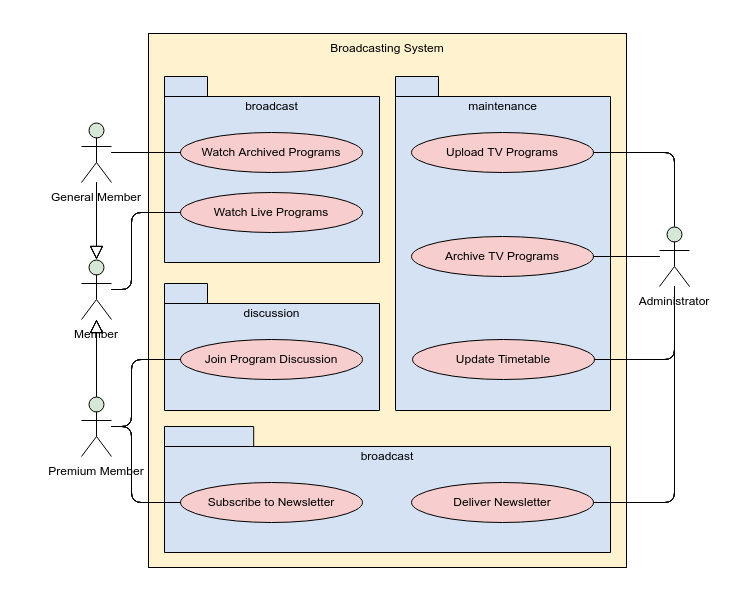
\includegraphics[scale=0.5]{Book-SSW565/png/UML Diagram.png} 
\end{figure}

\textbf{Broadcast System \gls{stakeholder}s:}
\begin{enumerate}
    \item System Administrator
    \item System Owner
    \item Viewer
\end{enumerate}

% Add a section and label it so that we can reference it later
\section{Applying Tactics of Availability \label{Section::Applying Tactics of Availability}}

\begin{longtable}{|l|p{12cm}|}
%\centering
\caption{\TableName{Quality Attribute: Availability} \TableLabel{QA: Availability} \label{Table::QA:Availability}}\\
    
    \hline
    \textbf{Portion} & \textbf{Possible Values}\\
    \hline 
    \endfirsthead

    \multicolumn{2}{c}{\tablename\ \thetable\ -- \textit{Continued from previous page}}\\
    \hline
    \textbf{Portion} & \textbf{Possible Values}\\
    \hline
    \endhead
    
    \multicolumn{2}{r}{\tablename\ \thetable\ -- \textit{Continued on next page}} \\
    \endfoot
    \endlastfoot

\gls{stakeholder} & System Administrator
\\ \hline

\gls{source} & Multiple requests, network failure, high traffic load
\\ \hline

\gls{stimulus} & Delay in response time, slow down system performance, unexpected server failure
\\ \hline

\gls{environment} & Normal Operation, System overloaded, network congestion, hardware failure
\\ \hline

\gls{artifact} & Load balancing system, redundant servers, monitoring tools
\\ \hline

\gls{response} & Detects, prevents, and recovers from faults by using tactics such as heartbeat monitoring, redundancy, load balancing, and fault recovery mechanisms
\\ \hline

\gls{responseMeasure} & System remains responsive within acceptable time limits, ensures minimal downtime by failing over to backup servers, retrying failed requests, and automatically adjusting resources (divide among multiple servers)
\\ \hline

\end{longtable}



\section{Applying Tactics of Performance\label{Section::Applying Tactics of Performance}}

\begin{longtable}{|l|p{12cm}|}
%\centering
\caption{\TableName{Quality Attribute: Performance} \TableLabel{QA: Performance} \label{Table::QA:Performance}}\\
    
    \hline
    \textbf{Portion} & \textbf{Possible Values}\\
    \hline 
    \endfirsthead

    \multicolumn{2}{c}{\tablename\ \thetable\ -- \textit{Continued from previous page}}\\
    \hline
    \textbf{Portion} & \textbf{Possible Values}\\
    \hline
    \endhead
    
    \multicolumn{2}{r}{\tablename\ \thetable\ -- \textit{Continued on next page}} \\
    \endfoot
    \endlastfoot

\gls{stakeholder} & System Administrator/Viewer
\\ \hline

\gls{source} & High incoming traffic, multiple concurrent viewer requests
\\ \hline

\gls{stimulus} & Increased latency, Increased response time, resource exhaustion
\\ \hline

\gls{environment} & Web application, cloud-based system, real-time processing, limited hardware resources
\\ \hline

\gls{artifact} & Application servers, databases, load balancers
\\ \hline

\gls{response} & Control resource demand (e.g., limit event response, prioritize events, reduce overhead) and Manage resources efficiently (e.g., introduce concurrency, schedule resources, maintain multiple copies of data, increase resources)
\\ \hline

\gls{responseMeasure} & Response generated within time constraints, optimized latency and throughput, and minimal resource wastage
\\ \hline

\end{longtable}
\chapter{Architecture Modeling with UML \\
\small{\textit{-- ZKD, KRV, CL, \& ZZ}}
\index{Architecture Modeling} 
\index{Chapter!ArchitectureModeling}
\label{Chapter::ArchitectureModeling}}

\section{CRC Cards}
\begin{description}
   
\subsection{Student Class}
\begin{center}
\begin{tabular}{|p{5cm}|p{5cm}|}
    \hline
    \textbf{Responsibilities} & \textbf{Collaborators} \\
    \hline
    - Attend class,  & School\\
      use a transport mode to go to & Bike \\
      school & Shoes \\
    \hline
\end{tabular}
\end{center}

\subsection{John Class}
\begin{center}
\begin{tabular}{|p{5cm}|p{5cm}|}
    \hline
    \textbf{Responsibilities} & \textbf{Collaborators} \\
    \hline
    - Ride a bike to school & School \\
    & Bike\\
    \hline
\end{tabular}
\end{center}

\subsection{Maria Class}
\begin{center}
\begin{tabular}{|p{5cm}|p{5cm}|}
    \hline
    \textbf{Responsibilities} & \textbf{Collaborators} \\
    \hline
    - Walk to school using shoes & School \\
     & Shoes \\
    \hline
\end{tabular}
\end{center}

\subsection{Shoes Class}
\begin{center}
\begin{tabular}{|p{5cm}|p{5cm}|}
    \hline
    \textbf{Responsibilities} & \textbf{Collaborators} \\
    \hline
    -Assist in walking to school & Maria \\
    \hline
\end{tabular}
\end{center}

\subsection{Bike Class}
\begin{center}
\begin{tabular}{|p{5cm}|p{5cm}|}
    \hline
    \textbf{Responsibilities} & \textbf{Collaborators} \\
    \hline
    - Provide a means of transportation & John \\
    \hline
\end{tabular}
\end{center}

\subsection{School Class}
\begin{center}
\begin{tabular}{|p{5cm}|p{5cm}|}
    \hline
    \textbf{Responsibilities} & \textbf{Collaborators} \\
    \hline
    - Receive students  & Student\\
    \hline
\end{tabular}
\end{center}
 \end{description}
 
\section{Use Case Diagram}
The \textbf{Use Case Diagram} was designed to illustrate how \textbf{John and Maria} interact with the system. It focuses on their different methods of transportation:
\begin{itemize}
    \item \textbf{John} uses a \textbf{bike} to reach class, represented as a direct use case of "Ride Bike."
    \item \textbf{Maria} follows a \textbf{two-step process}: first, she wears shoes, then she walks to class. This dependency is depicted by linking the "Wear Shoes" and "Walk to Class" use cases.
    \item \textbf{Actors} (John and Maria) interact only with their respective transportation methods, ensuring a clear and simple flow.
\end{itemize}
This diagram effectively captures the \textbf{functional perspective} of how students go to school.

\begin{figure}[H]
    \centering
    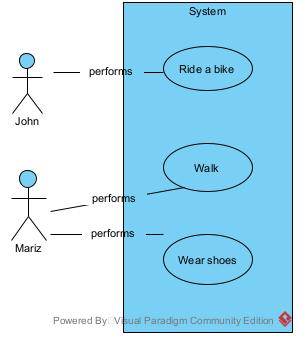
\includegraphics[scale=0.75]{Book-SSW565/jpg/ArchitectureModeling/Use Case Diagram1.jpg}
    \caption{\label{Figure::Use Case Diagram}Use Case Diagram}
\end{figure}


\section{Object Diagram}
The \textbf{Object Diagram} models a \textbf{specific scenario} of the user story. It represents actual instances of the classes at a given moment:
\begin{itemize}
    \item \textbf{John's Bike} is \textbf{directly associated} with him.
    \item \textbf{Maria owns shoes}, which she \textbf{needs for walking}.
    \item The \textbf{relationship between objects} is crucial: Maria \textbf{cannot walk without shoes}, reinforcing \textbf{dependency}.
    \item \textbf{Multiplicities} (one-to-one associations) are implied in the relationships to reflect real-world constraints.
\end{itemize}

The thought process behind this diagram was to provide \textbf{a snapshot} of how objects interact in the real world, helping to validate the correctness of the class relationships before formalizing them in the \textbf{Class Diagram}.

\begin{figure}[H]
    \centering
    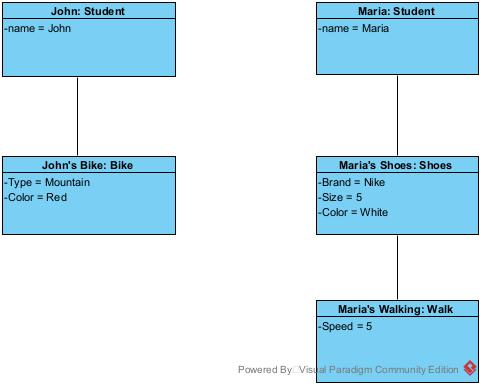
\includegraphics[scale=0.75]{Book-SSW565/jpg/ArchitectureModeling/Object Diagram1.jpg}
    \caption{\label{Figure::Object Diagram}Object Diagram}
\end{figure}

\section{Class Diagram}
The \textbf{Class Diagram} is the most detailed and structured representation of the system. It was designed using \textbf{three key relationships}:
\begin{itemize}
    \item \textbf{Generalization (Inheritance):} \texttt{Bike} and \texttt{Shoes} are both types of \texttt{TransportMode}, making use of \textbf{inheritance} to reduce redundancy.
    \item \textbf{Generalization (Inheritance):} \texttt{John} and \texttt{Maria} are both types of \texttt{Student}, making use of \textbf{inheritance} to reduce redundancy.
    \item \textbf{Aggregation:} A \texttt{Student} \textbf{uses} a \texttt{TransportMode} method but does not permanently own it (represented with a \textbf{hollow diamond}).
    \item \textbf{Composition:} \texttt{Student} \textbf{requires} \texttt{School} (depicted with a \textbf{filled diamond}), meaning a \texttt{Student} instance \textbf{cannot exist} without \texttt{School}.
\end{itemize}

This diagram refines the \textbf{structure of the system} by making clear distinctions between \textbf{inheritance, dependencies, and ownership relationships}, forming the blueprint for implementing the system in code.


\begin{figure}[h]
    \centering
    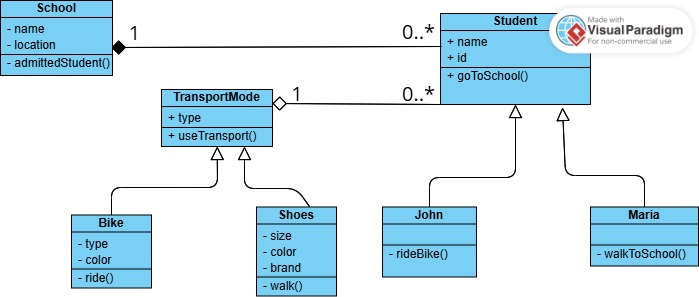
\includegraphics[scale=0.6]{Book-SSW565/jpg/ArchitectureModeling/Class_Diagram.jpg}
    \caption{\label{Figure::Class Diagram}Class Diagram}
\end{figure}


\chapter{Usability, Security, Safety and Energy Efficiency \\
\small{\textit{-- ZKD, KRV, CL, \& ZZ}}
\index{Usability, Security, Safety and Energy Efficiency} 
\index{Chapter!Usability}
\label{Chapter::Usability}}

\textbf{Context:} The oscilloscope is networked and shares data with labs that may be interested in remote monitoring of voltages.  The oscilloscope has a Wi-Fi and cellular connection.

\begin{figure}[h]
    \centering
    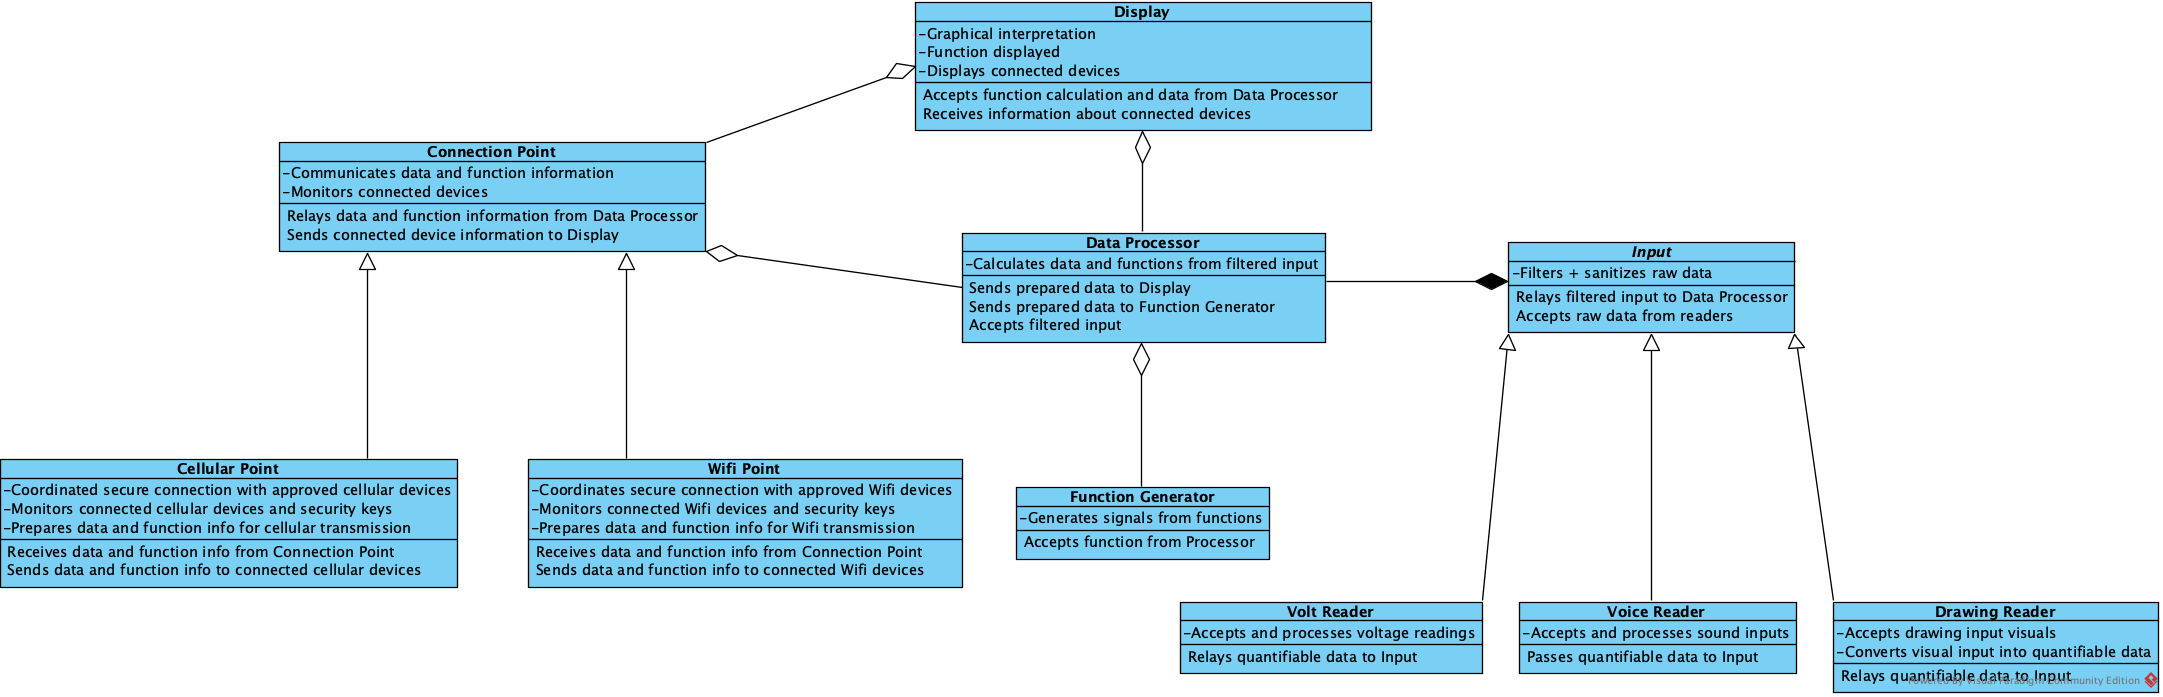
\includegraphics[scale=0.4]{Book-SSW565/png/Scope-Function-Generator-2.png}
    \caption{\label{Figure::Oscilloscope Class Diagram}Oscilloscope Class Diagram}
\end{figure}

\section{Usability Scenario}

\begin{longtable}{|l|p{12cm}|}
%\centering
\caption{\TableName{Usability Scenario for Oscilloscope} \TableLabel{USOscilloscope} \label{Table::UsabilityOscilloscope}}\\
    
    \hline
    \textbf{Portion} & \textbf{Possible Values}\\
    \hline 
    \endfirsthead

    \multicolumn{2}{c}{\tablename\ \thetable\ -- \textit{Continued from previous page}}\\
    \hline
    \textbf{Portion} & \textbf{Possible Values}\\
    \hline
    \endhead
    
    \multicolumn{2}{r}{\tablename\ \thetable\ -- \textit{Continued on next page}} \\
    \endfoot
    \endlastfoot

\gls{stakeholder} & Lab Engineer / Technician
\\ \hline

\gls{source} & The engineer initiates the action via a web-based interface or a mobile app connected to the oscilloscope.
\\ \hline

\gls{stimulus} & The engineer logs in and selects the volt reader function, then modifies the voltage either Vertical scale (volts per division) or Vertical scale (volts per division).
\\ \hline

\gls{environment} & The oscilloscope is in a networked lab environment, accessed remotely by Wi-Fi or cellular network.
\\ \hline

\gls{artifact} & The oscilloscope system, including the Wi-Fi Point, Cellular Point, Volt Reader, and Data Processor, which must authenticate the user before allowing adjustments.
\\ \hline

\gls{response} & The oscilloscope authenticates the user, then applies the voltage change, updating the display with the new settings.
\\ \hline

\gls{responseMeasure} & Authentication time less than and equal to 15 sec \\
     & Voltage adjustment processing time less than and equal to 5 sec \\
     & Total time for task completion less than and equal to 20 sec
\\ \hline

\end{longtable}
An engineer remotely accesses the networked oscilloscope, requiring authentication before voltage settings can be altered. The system then processes the change and updates the display. Performance is measured by total interaction time and system response speed.

\section{Usability Trade-offs}
While usability is a great improvement to any software, the trade-offs of such need to be considered in the full scope of the system. Depending on the system and its trade-offs, the developers need to find a healthy balance.

\subsection{Against Security}
The trade-off between usability and security tends to be that as the software gets more user friendly, detailed options might start to be removed for the user's experience which can lead to a less secure connection. Think of it this way, the easier it is for someone to connect their device to the oscilloscope, the easier it is for anyone to connect their device to that same oscilloscope and read all the data being transmitted. While yes, the oscilloscope has become easier to use, it also compromises the possible sensitive data from the device or the other devices connected to it. 
\paragraph{\textbf{The above-mentioned scenario significantly impacts security:}}
\begin{itemize}
    \item Without authentication: Instant access (around ~5 sec).
    \item With authentication: Extra 10-15 sec before access.
\end{itemize}

\begin{table}[htbp]
\centering
\caption{Usability, Security, and Access Time Comparison}
\resizebox{\textwidth}{!}{
\begin{tabular}{|l|c|c|c|} % Added vertical bars
\hline % Added top border
\textbf{Scenario} & \textbf{Usability Impact} & \textbf{Security Benefit} & \textbf{Access Time} \\
\hline % Added horizontal line
No Authentication & Fast access (around 5 sec) & Unprotected, anyone can access & around 5 sec \\
\hline
Authentication Required & Slower access (15-20 sec) & Secure, only authorized users & 15-20 sec \\
\hline % Added bottom border
\end{tabular}}
\label{tab:security_usability}
\end{table}

\paragraph{\textbf{Solution of above trade-offs:}}
 Implement a "Remember Me" feature to reduce login time for returning users.

\subsection{Against Performance}
Trade-offs between usability and performance may system from a developer's desire to keep the oscilloscope very simple to use while still accounting for all possible use cases of said machine. That means that while the user might only want to read the voltage of something and have it displayed on the Display, the software might take all possible functions and features into account, such as preparing that data for WiFi transmission, which compromise performance. 

\paragraph{\textbf{The above-mentioned scenario significantly impacts performance:}}
\begin{itemize}
    \item If oscilloscope encrypts data before sending via Wi-Fi, it might delay response times by 1-2 sec.
    \item If Data Processor filters raw input before calculation, it ensures accuracy but adds processing time.
\end{itemize}
\paragraph{\textbf{Solution through Optimization:}}Perform real-time processing in parallel with data transmission.

\section{Requirements}

\subsection{Requirement 1: Voltage Measurement and Adjustment}
The oscilloscope must provide precise \textbf{voltage measurement} and allow users to adjust the \textbf{either Vertical scale (volts per division) or Vertical scale (volts per division).} remotely via a web-based interface or mobile app.

\paragraph{\textbf{Usability Response:}}  
The oscilloscope authenticates the user, then applies the voltage change, updating the display with the new settings.

\paragraph{\textbf{Response Measure:}}  
\begin{itemize}
    \item Authentication time: $\leq 15$ seconds.
    \item Voltage adjustment processing time: $\leq 5$ seconds.
    \item Total task completion time: $\leq 20$ seconds.
\end{itemize}

\paragraph{\textbf{Comparison of Usability:}}  
Compared to traditional oscilloscopes, which require physical interaction for voltage adjustments, this remote-controlled oscilloscope improves usability by allowing engineers to make real-time changes from anywhere. The inclusion of authentication ensures security, but it adds a minor delay in response time. The \textbf{automated process reduces human error} while maintaining efficiency.

\subsection{Requirement 2: Frequency Measurement and Remote Monitoring}
The oscilloscope must allow users to measure \textbf{signal frequency} and remotely monitor real-time waveforms over Wi-Fi and cellular networks.

\paragraph{\textbf{Usability Response:}}  
The oscilloscope captures and transmits frequency data to remote users, allowing them to view measurements in real-time.

\paragraph{\textbf{Response Measure:}}  
\begin{itemize}
    \item Frequency detection processing time: $\leq 10$ milliseconds.
    \item Data transmission time to remote labs: $\leq 3$ seconds.
    \item Display update interval: $\leq 1$ second.
\end{itemize}

\paragraph{\textbf{Comparison of Usability:}}  
Traditional oscilloscopes require engineers to be physically present for monitoring. The ability to view frequency readings remotely enhances usability by allowing multiple users to access data from different locations. However, data transmission over a network introduces slight latency, which could be an issue in high-precision applications.  

\section{Energy Trade-offs}

\paragraph{\textbf{Wi-Fi Point:}}  
\begin{itemize}
    \item Lower power consumption compared to cellular.
    \item Requires authentication for every new session, adding a slight delay.
    \item More stable connection in controlled lab environments.
    \item Limited range, requiring the user to be within the Wi-Fi coverage area.
\end{itemize}

\paragraph{\textbf{Cellular Point:}}  
\begin{itemize}
    \item Higher power consumption due to continuous network communication.
    \item Allows persistent connections, reducing the need for frequent re-authentication.
    \item Greater range, enabling remote access from anywhere with a cellular network.
    \item Potential latency issues, depending on network conditions.
\end{itemize}

\paragraph{\textbf{Define better way to improve energy efficiency:}}  
\begin{itemize}
    \item Use Wi-Fi for frequent, short-duration access to conserve energy.
    \item Use Cellular for long-term remote monitoring where stability and persistent access are prioritized.
    \item Implement adaptive authentication (e.g., session-based authentication caching) to balance usability, security, and energy efficiency.
\end{itemize}




\chapter{Architecture Patterns \\
\small{\textit{-- ZKD, KRV, CL, \& ZZ}}
\index{Architecture Patterns} 
\index{Chapter!Architecture Patterns}
\label{Chapter::Architecture Patterns}}

\section{Search Engine}
Assuming we have a very large dataset of shoes with various brands, styles, colors and sizes like Zappos \cite{zappos} does, we need to figure out which architectural pattern should be applied for basic search engine capability of our enormous dataset.

\subsection{Pipe and Filter Pattern}
For a basic search engine to handle a large dataset of shoes (brands, styles, colors, sizes), the Pipe and Filter Pattern is an excellent fit.

\subsection{Why Pipe and Filter?}
\begin{itemize}[leftmargin=*, label={\textbullet}]
    \item \textbf{Context}: You need to transform and process streams of data (search queries and shoe datasets) in a modular, scalable way.
    
    \item \textbf{Problem}: The system needs to be divided into reusable, loosely coupled components that can be flexibly combined and scaled.
    
    \item \textbf{Solution}: Pipe and Filter allows for data to be processed in filters, with each filter handling a specific part of the search query---like filtering by brand, style, color, or size---and outputting refined results down the line.
\end{itemize}

\begin{figure}[h]
    \centering
    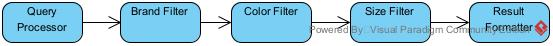
\includegraphics[scale=0.7]{Book-SSW565/jpg/ArchitecturePatterns/Pipe and Filter.jpg}
    \caption{\label{Figure::Pipe and Filter}Pipe and Filter}
\end{figure}

\subsection{Component and Connector Pattern}
To support user access to the search engine, the Client-Server Pattern (from the Component and Connector patterns) is a great choice. It enables the system to support multiple users searching for shoes concurrently, with the server side managing and processing requests. Client-Server to provide user access and support distributed users interacting with the system.

\begin{figure}[h]
    \centering
    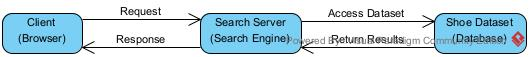
\includegraphics[scale=0.7]{Book-SSW565/jpg/ArchitecturePatterns/Component and Connector Pattern.jpg}
    \caption{\label{Figure::Component and Connector Pattern}Component and Connector Pattern}
\end{figure}

\section{Model View Controller}
\begin{lstlisting}[caption=model.py]
# model.py
class User:
    def __init__(self, name, age):
        self.name = name
        self.age = age

class UserModel:
    def __init__(self):
        self.users = []  # Simulating a database

    def add_user(self, name, age):
        user = User(name, age)
        self.users.append(user)

    def get_users(self):
        return self.users
\end{lstlisting}
\begin{lstlisting}[caption=view.py]
# view.py
class UserView:
    def __init__(self):
          pass # good for a breakpoint

    @staticmethod
    def show_users(users):
        print("\nUser List:")
        for user in users:
            print(f"Name: {user.name}, Age: {user.age}")

    @staticmethod
    def show_message(message):
        print(message)
\end{lstlisting}

\begin{lstlisting}[caption=controller.py]
# controller.py
from model import UserModel
from view import UserView


class UserController:
    def __init__(self):
        self.model = UserModel()
        self.view = UserView()

    def add_user(self, name, age):
        self.model.add_user(name, age)
        self.view.show_message(f"User '{name}' added successfully!")

    def display_users(self):
        users = self.model.get_users()
        self.view.show_users(users)


# Run the MVC
if __name__ == "__main__":
    controller = UserController()

    controller.add_user("Alice", 25)
    controller.add_user("Bob", 30)

    controller.display_users()

\end{lstlisting}

\subsection{Class Diagram}
\begin{figure}[H]
    \centering
    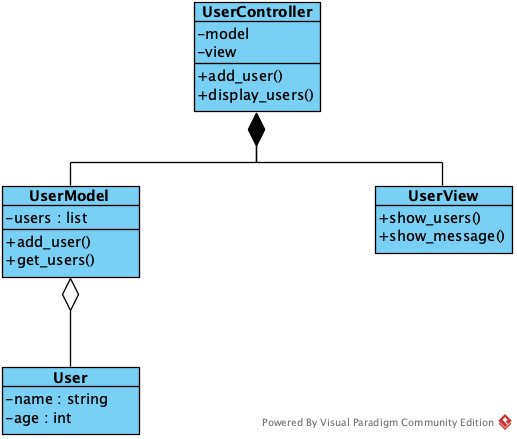
\includegraphics[scale=0.8]{Book-SSW565/jpg/ArchitecturePatterns/MVC Class Diagram.png}
    \caption{\label{Figure::MVC Class Diagram}MVC Class Diagram}
\end{figure}

\subsection{Object Diagram}
\begin{figure}[H]
    \centering
    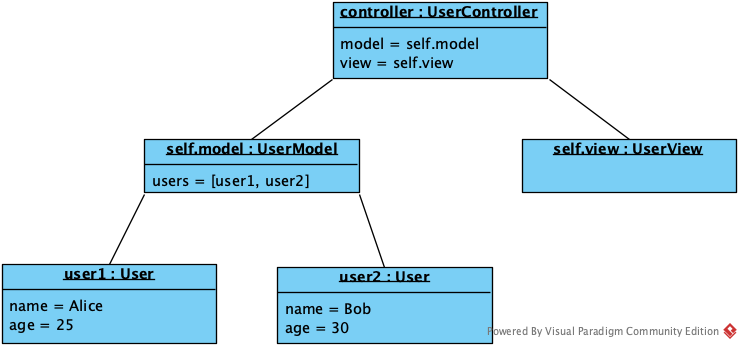
\includegraphics[scale=0.7]{Book-SSW565/jpg/ArchitecturePatterns/ScenarioObjectDiagram.png}
    \caption{\label{Figure::MVC Object Diagram}MVC Object Diagram}
\end{figure}

\subsection{Sequence Diagram}
\begin{figure}[H]
    \centering
    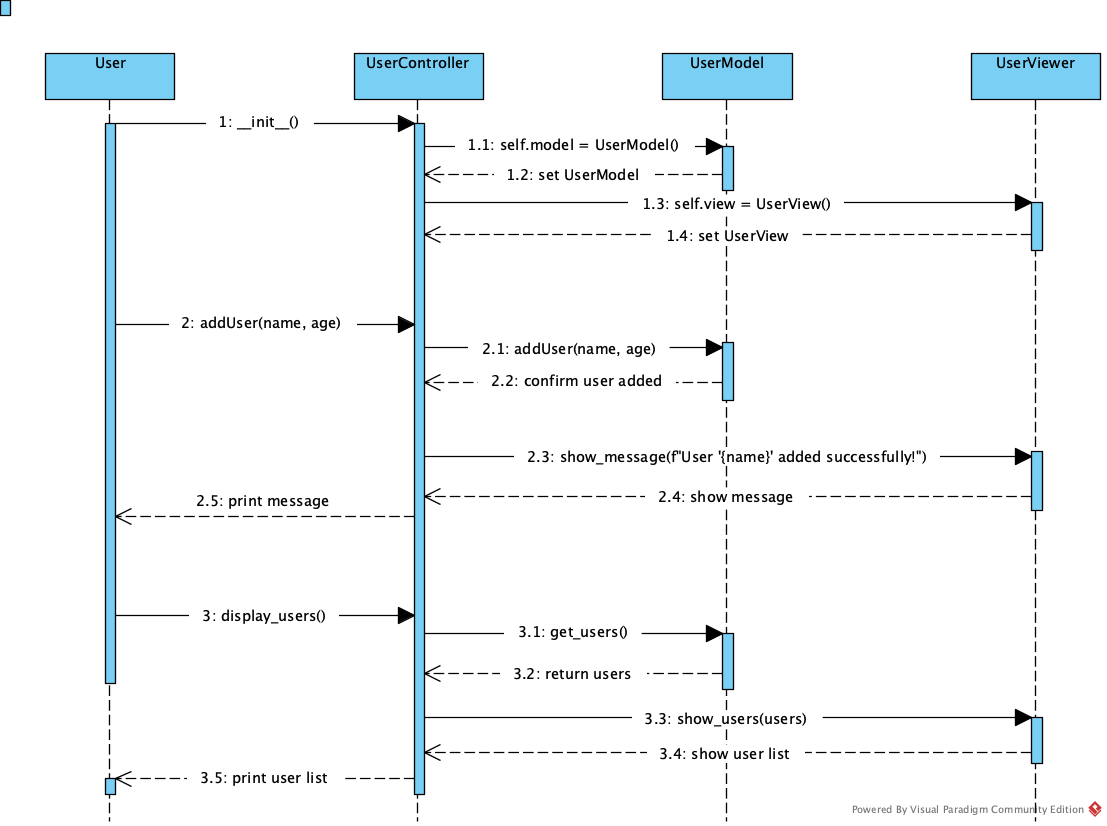
\includegraphics[scale=0.7]{Book-SSW565/jpg/ArchitecturePatterns/MVCSequenceDiagram.png}
    \caption{\label{Figure::MVC Sequence Diagram}MVC Sequence Diagram}
\end{figure}


\section{In-Class Exercise: Redesigned Oscilloscope}
Redesigning the Oscilloscope using the "MVC" for the user interface and "Pipe and Filter" for the signal processing part. Assuming that the two filters we have are: scpScale (to scale the signal) and scpOffset to offset the signal.

\subsection{MVC and Pipe-Filter Patterns}
\begin{enumerate}
  \item  \textbf{Model-View-Controller (MVC) for Oscilloscope UI}
  \newline \textbf{Description:}
    \begin{itemize}
        \item  \textbf{Model:}
        \newline Represents Oscilloscope data.(waveforms, voltage readers, etc.)
        \item \textbf{View:}
        \newline Handles display functions.
        \item \textbf{Controller:}
        \newline Manages user interaction and updates the model.
    \end{itemize}
  \item \textbf{Pipe and Filter Pattern for Signal Processing}
  \newline \textbf{Description:}
  \newline The Pipe and Filter pattern is used to process oscilloscope signals through a sequence and parallel of operations.
  \begin{itemize}
      \item \textbf{Filters:}
      \newline Modify signal data (scaling, offset adjustments).
      \item \textbf{Pipes:}
      \newline Pass the transformed signal between filters. or Perform parallel work by filters on the raw waveform data.
  \end{itemize}
  In the oscilloscope redesign using the Pipe and Filter pattern, we can incorporate parallel processing where applicable.
  \newline \textbf{Parallel Approach:}
  \begin{itemize}
      \item We consider scpScale and scpOffset are not depend on each other's results, they can be processed simultaneously in parallel.
      \item The raw input signal is split and sent to both filters at the same time.
      \item After both filters finish processing, the results are merged back before passing to the display.
  \end{itemize}
\end{enumerate}

\subsection{Class Diagram}
\subsection{Object Diagram}
\subsection{Sequence Diagram}

\appendix
\chapter{Homework Assignments \\
\small{\textit{-- From Canvas}}
\index{Homework Assignments} 
\index{Appendix!Homework}
\label{Appendix::Homework}}

These are the group assignments listed on the Canvas course for SWW 564-A in chronological order. Each of these assignments includes all aspects, requirements, and bullets directly from the assignment.

%----------------------------------------------------------------------------------------
%-------------------------------------- HOMEWORK 4 --------------------------------------
%----------------------------------------------------------------------------------------
\section{Assignment 4 \textit{-- Applying Tactics of Availability and Performance}}\label{Assignments::4}
\textbf{Due:} February 24th, 2025 \\

\noindent
To complete this assignment, use chapters 4 and 9 of your textbook,

\begin{enumerate}
    \item In your work group, reuse, modify or add quality attributes scenarios of Availability and Performance in "#3 Quality Attributes -- Individual", propose appropriate tactics for achieving any of desired qualities.  
    \item Prepare and submit your proposals using the Overleaf manual template and add a new chapter titled "Applying Tactics of Availability and Performance."  Please reference all authors and save the homework into a new file that you will add to the project.  Call it <xyz>AvailabilityAndPerformance.tex, where <xyz> is your team's name space.
    \item Update the document history and clean up any chapters from the old template given to you.
\end{enumerate}
%----------------------------------------------------------------------------------------
%-------------------------------------- HOMEWORK 4b --------------------------------------
%----------------------------------------------------------------------------------------
\section{Assignment 4b \textit{-- Architecture Modeling with UML}}\label{Assignments::4b}
\textbf{Due:} February 24th, 2025 \\

\noindent
You are to design a software program that simulates a simple process of students going to school in the morning. You are given the following user story: John and Maria are two students at Stevens Institute of Technology, a local university. John gets to his classes by riding his bike and Maria gets to her class by putting on her shoes and walking to class. \\

\noindent
Model the above user story using the following modeling techniques:

\begin{enumerate}
    \item Create CRC cards depicting all the possible classes in the user story and extracting the CRC cards. For each CRC card make sure you describe the responsibilities and collaborations with the other classes (cards).
    \item Create a use case diagram, depicting the user story.
    \item Create an object diagram, depicting the exact scenario of the user story. Show all the associations.
    \item From the object diagram create a class diagram. Add as many association multiplicities and label any association ends as completely as you can. Make use of the following three association types: aggregation, composition, and generalization. This may require that you think of additional subclasses, in addition to the classes that the user story provided to you. You can use more than the three associations given above.

    Add at least one paragraph describing the thought process for each of the three diagrams. There is no right or wrong answer for this exercise. You will be graded on the completeness of your solution.
    \item Update your history table (\ref{Table::UpdateHistory}) and make sure you are generating a clean document, with a new chapter for this assignment. Up to 10 points are taken away for documents that are not "clean and organized."
\end{enumerate}
%----------------------------------------------------------------------------------------
%-------------------------------------- HOMEWORK 5 --------------------------------------
%----------------------------------------------------------------------------------------
\section{Assignment 5 \textit{-- Usability, Security, Safety and Energy Efficiency}}\label{Assignments::5}
\textbf{Due:} March 3rd, 2025 \\

\noindent
To your Overleaf Group Project, add a new chapter and title it: Usability, Security, Safety and Energy Efficiency.

\begin{enumerate}
    \item The oscilloscope is networked and shares data with labs that may be interested in remote monitoring of voltages.  The oscilloscope has a Wi-Fi and cellular connection.
    \item Write a concrete usability scenario for your Oscilloscope that specifies how long it takes you to adjust some aspect of the oscilloscope. Now consider another part of the user experience and create scenarios that test other aspects of the response measures from the general scenario table. (25 points)
    \item How might usability trade-off again security? How might it trade-off against performance? (25 points.)
    \item Pick two of the requirements of the Oscilloscope (i.e. voltage measurement, frequency measurement, peak-to-peak detection, something else) . Pick one appropriate response from the usability general scenario and an appropriate corresponding response measure. Use the response and response measure you chose, compare the scope's usability.  (25 points)
    \item What are the energy tradeoffs in your Oscilloscope between using Wi-Fi and the cellular network? (25 points)
    \item Please reference any outside sources with \verb|\cite{}| and add them to the bibliography file and please add at least 10x new \verb|\index{}| terms in this assignment.  You can add more, if you'd like.
\end{enumerate}
%----------------------------------------------------------------------------------------
%-------------------------------------- HOMEWORK 6a --------------------------------------
%----------------------------------------------------------------------------------------
\section{Assignment 6a \textit{-- Architecture Patterns}}\label{Assignments::6a}
\textbf{Due:} March 10th, 2025 \\
\begin{enumerate}
    \item Create a new chapter in your Overleaf/LaTeX manual and call it: Architecture Patterns.
    \item Add a \verb|\cite{}| to the Bibliography and reference the video link from above.
    \item Watch the video on the Zappos Systems Architecture found in this week's Module on Canvas.  Like Zappos, suppose that you have a very large dataset of shoes with various brands, styles, colors and sizes. In the chapter answer and expand on the following questions:
    \begin{enumerate}
        \item Which pattern should be applied for a a basic search engine capability for your dataset of shoes? Explain why this pattern should be applied.  Include at least one block diagram of your design.
        \item Place your search engine design within a component and connector pattern that could be used to support user access and prepare a brief description of your overall design.
    \end{enumerate}
    \item Using the code from MVC.zip
    \begin{enumerate}
        \item Create the UML diagram of the MVC files
        \item Create an sequence diagram that depicts the sequence of events in the main() program.  Make sure you set break-points and step through the program to clearly map all the function calls.
    \end{enumerate}
    \item \textbf{In class exercise:} Redesign the Oscilloscope using the "MVC" for the user interface and "Pipe and Filter" for the signal processing part.  Assume that the two filters we have are: scpScale (to scale the signal) and scpOffset to offset the signal.  Provide a UML diagram class diagram of the new design.  Use the standard associations: inheritance, composition, aggregation, and label any other associations by name.  Use multiplicities, too.
\end{enumerate}




% makeglossaries dsnManual -- from command prompt.
\clearpage
%\printglossaries
\printnoidxglossaries

\bibliography{bibfile}
%\bibliographystyle{unsrt}
\bibliographystyle{IEEEtran}

\printindex
%\input{dsnManual.idx}
\end{document}
